\subsection{Project overview}
The principal idea is that GNSS in together with other sources act as data providers to our AI module, which will collect and integrate this information to its algorithm. Next, the AI module will output a prediction of key parameters, that will be later interpreted and made understandable for agricultors. This part is where ARIFI specially stands out from other services, as it will make special emphasis in translating AI predictions into actions to take from farmers, so that their harvest follows a more efficient agricultural plan. In figure \ref{fig:sch1}, it is displayed an schematic idea of ARIFI's general concept.
\begin{figure}[h!]
    \centering
    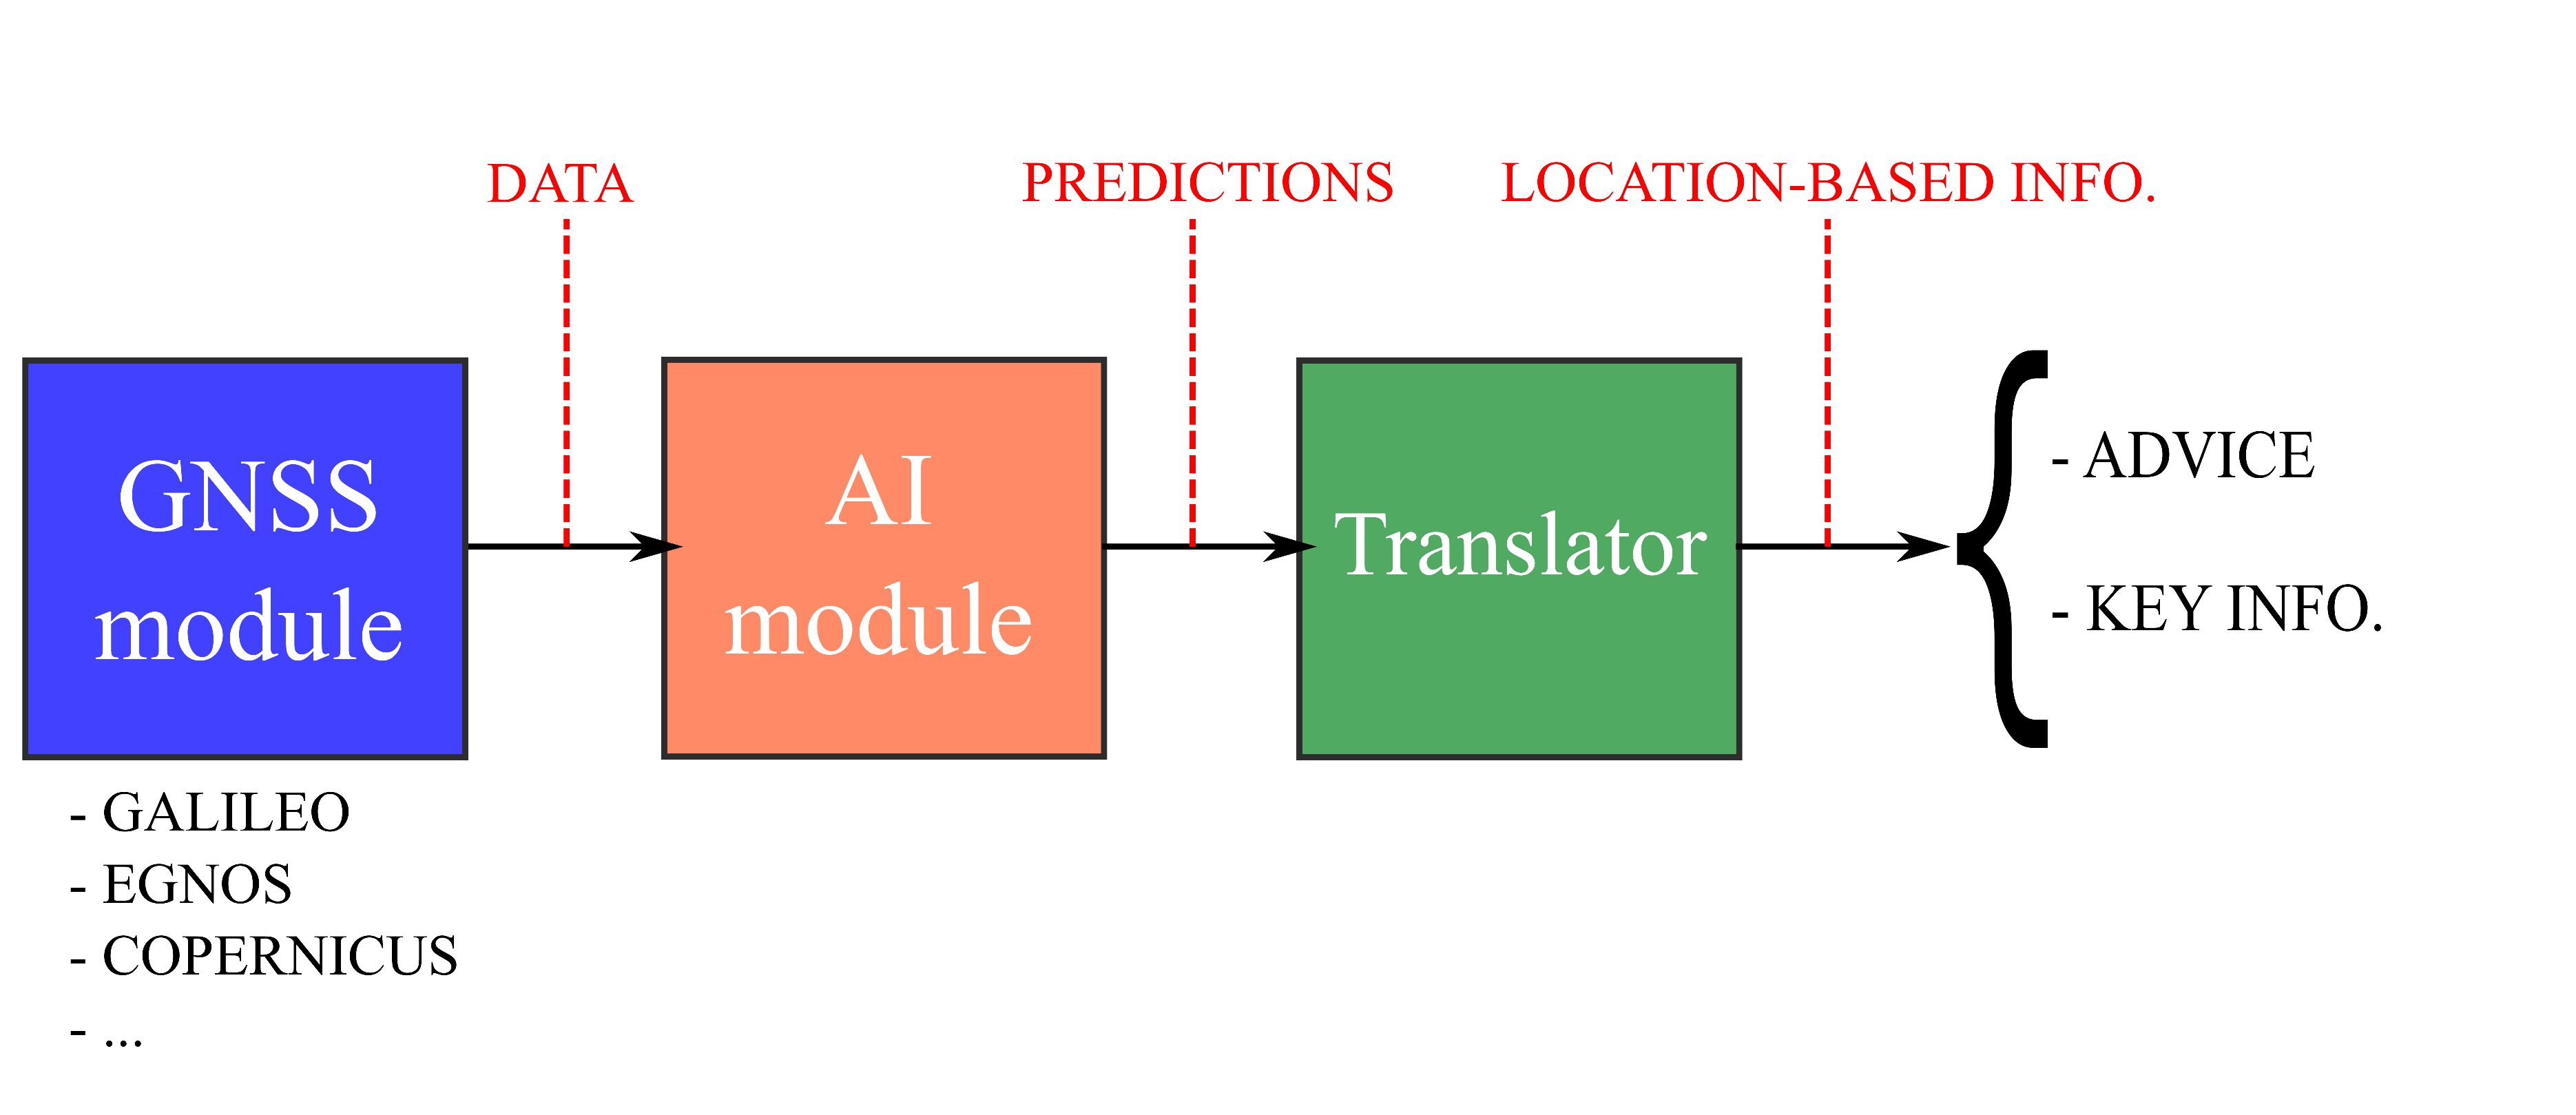
\includegraphics[scale= 0.26]{images/dibujo1.eps}
    \caption{ARIFI's general schematic}
    \label{fig:sch1}
\end{figure}\\\\
%
%
\begin{figure}[h!]
    \centering
    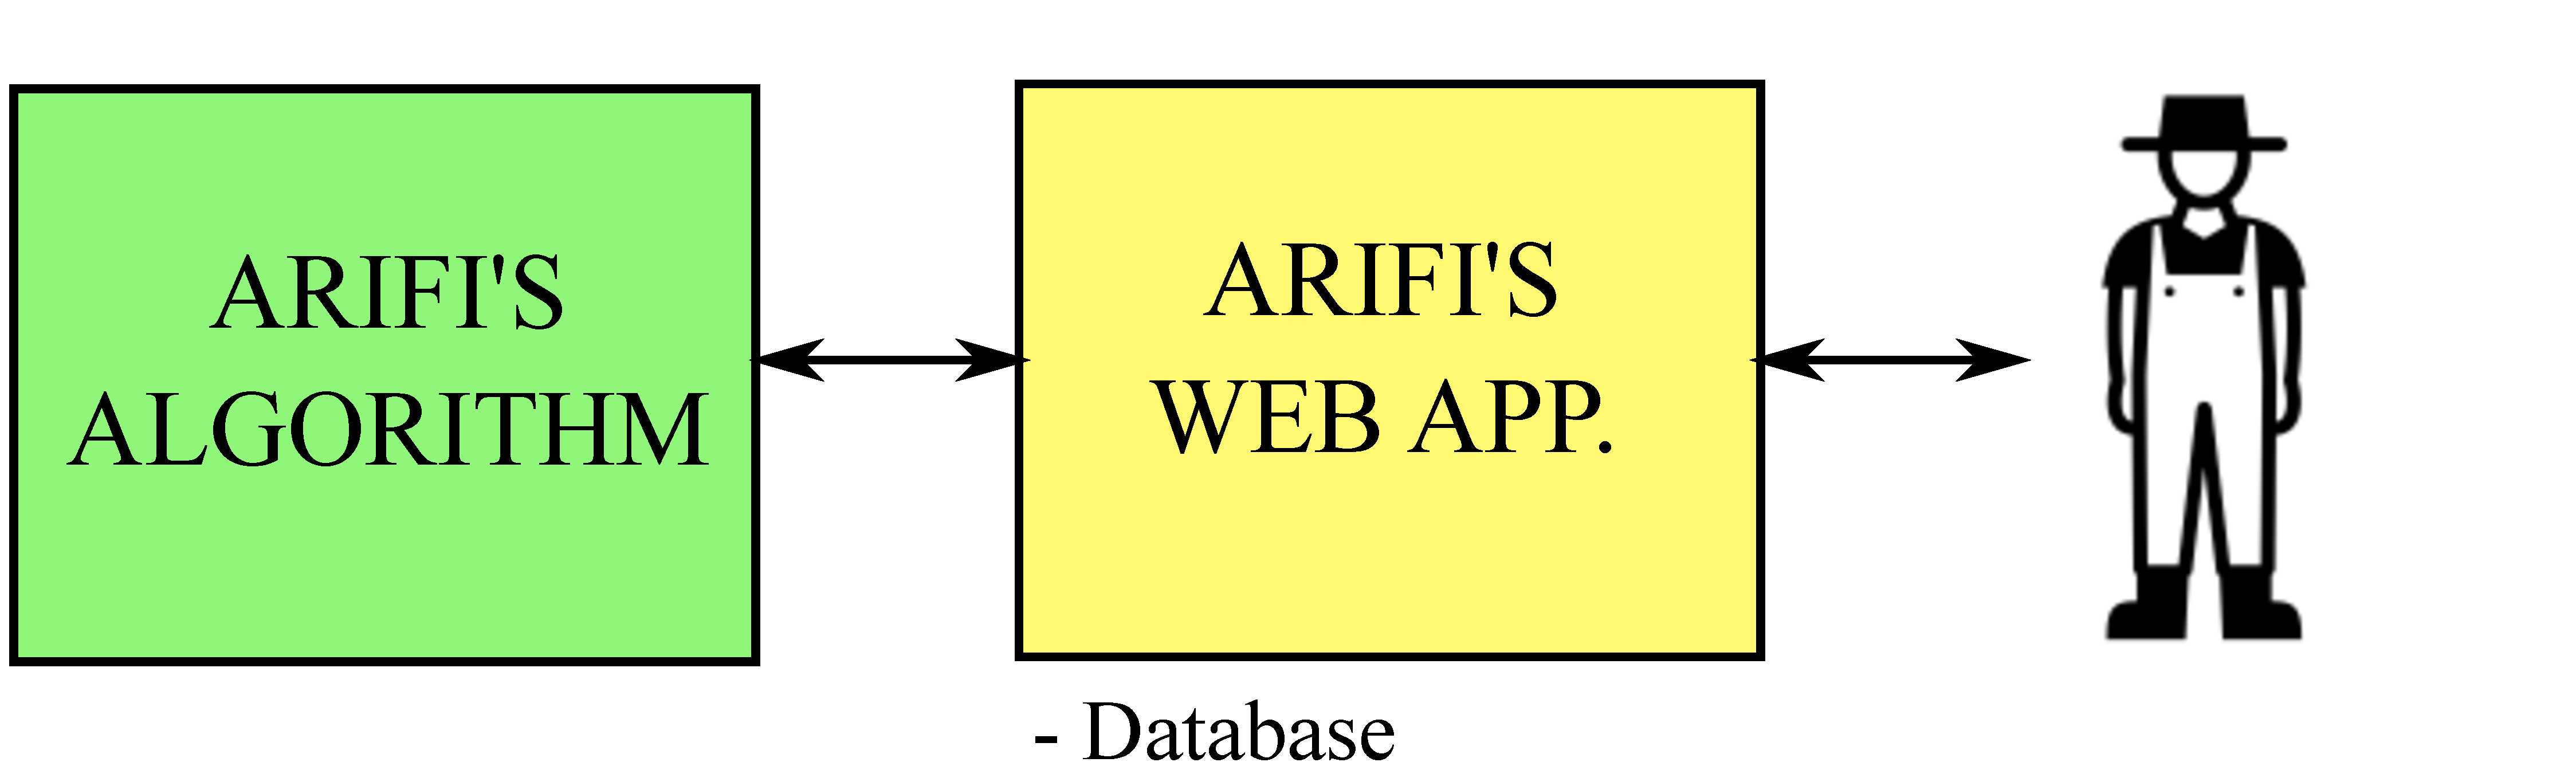
\includegraphics[scale= 0.20]{images/dibujo2.eps}
    \caption{User interaction with ARIFI's services}
    \label{fig:sch2}
\end{figure}
ARIFI was initially thought to work as a web application. The reason to this is that one of the major concerns from ARIFI's team, was to make this service available for a wide range of users. With this in mind, a web application was thought the best platform to work with, as it only requires a device with internet connection to access to its services. Despite this, we are opened to consider other platforms such as mobile-phone applications in the future. A graphical description of user's interaction with ARIFI is depicted in figure \ref{fig:sch2}.
